\chapter{Experiments on Synthetic Data}
\section{Setup}
\label{experiments}
\subsection{Initialization}
An important factor for online change point methods is determining how to initialize the algorithm. Because we are running an unsupervised model for classifying change points, we do not spend time training the model or tuning any of the hyperparameters. This is a double-edged sword because on one hand, we can drop in a change point algorithm onto a data stream and let it start running without much interference. On the other hand, if it does not have any prior distribution to compare to then it will need to be adjusted to know what's an appropriate reference or in-control distribution. This is usually referred to as the initialization phase for online algorithms.

There are many ways to get through the initialization step and create an appropriate reference sample. One way is to initially compare the oncoming data stream with some zero valued data. As data comes in, the algorithm can replace the reference data with real observations, creating a reference distribution. While this does assume that the data is initially in-control, it does provide a simple way to create a reference distribution on the fly without prior knowledge. When analysing the results, the practitioner must exclude the initial phase when comparisons were done with the initial zero values because the test statistic calculated from them will be insignificant. 

Another method is to construct the reference distribution with past data that do not contain change points if it is available as done in \cite{li2015m} and \cite{flynn2019change}. This method benefits from not having to spend time initializing the algorithm since it can immediately provide an informed statistical comparison. If the data stream is not very long or costly to acquire then this method is beneficial because the entire signal is retained.  On the other hand, prior work needs to be done to construct this sample and this may not always be feasible in practice. Another possible issue is what if the regime of the in-control distribution shifts to a new normal? Then the old reference distribution is no longer applicable and must be recreated again, which may be costly. 

\subsection{Structuring the Data Stream}
In practice, there is no universal way for evaluating online change point models given the nature of the problem. There are two main reasons for this. First, because change point detection originated in the statistical literature, most algorithms or models have strong theoretical results but have not being applied to synthetic or real datasets. Being able to handle high dimensional data streams is a relatively new benefit that has not been so research up until the mid-90's was largely theoretical in nature. Second, it's not obvious how an infinite data stream should be simulated to evaluate the efficacy of an algorithm. How long does synthetic data stream have to be to objectively evaluate an algorithm?  How can you actually know where change points occurred in a real dataset that has no obvious ground truth? It is not obvious how to answer these questions, nor does there exist a universal answer. Like most things, the answer depends on the context and what a practitioner is aiming to test with their particular algorithm.  

For this thesis, we wish to compare several methods not just one novel method, therefore data consistency and reproducibility will be important for drawing conclusions about performance. Synthetic datasets are a good way to replicate different distributions over and over. Real change points can also be exactly identifiable and compared to with synthetic data. Take for example a data stream where a single random variable is sampled from a normal distribution $\mathcal{N}(0,1)$ that incurs a change point and becomes a random variable from a normal $\mathcal{N}(0,2)$. I can control both of these distributions and know exactly where the change point occurred, but how should I determine how many observations should be observed before switching distributions? How many observations after the change point should I draw from the new distribution before realizing the algorithm will never detect this change point? Again, decisions like this are arbitrary and nuanced for evaluating online change point models because there is no universal method. 

We choose to

\subsection{Synthetic Datasets}
A common difficulty in change point detection is evaluating the performance of an algorithm with datasets that aren't overly simplistic and difficult enough to ascertain some real world use.

Unlike fields like image recognition where standardized datasets like MNIST provide a common benchmark, there are no standard datasets that are widely used across the change point detection literature for evaluating new methods. Most papers propose experiments that are relevant for the specific problem they are trying to solve  but lack examples or explanations of when their method would not be applicable.  Furthermore, because change point evolved out of the statistics literature, many papers focus on theoretical results and provide minor experimental results, if any.

Given the empirical focus of this thesis, we attempt to put together the most comprehensive experiments using synthetic data. To the best of our knowledge, no change point detection paper covers as many variations as presented in this thesis. While synthetic datasets are idealistic in their formulation, they provide a good starting point for comparing different methods because the exact location of the change points can be controlled for. This is a luxury that is often not available with real world datasets, making it difficult to ascertain performance on them. Therefore, to compare several kernel change point detection methods, they will be evaluated across several synthetic datasets.

Inspired by recent papers \cite{chang2019kernel} and \cite{flynn2019change} that attempt to bridge the gap between the statistics and machine-learning literature, we put together various challenging changes in distribution that may be encountered in a data stream. They are the following: change in mean, scaling variance, alternating between a Gaussian distribution and a Gaussian mixture, alternating between Gaussian mixtures, and alternating between Gaussian distribution and Laplace distribution. It is truly hard to properly generalize all the possible situations a non-parametric algorithm may be used in, but the synthetic cases presented in this thesis cover a range of applications. The following paragraphs describe how each one is constructed in detail.

For a change in mean, a change point is inserted in the time series at some random time where the mean is shifted either positively or negatively. There are two variants to this scenario. In the first, the mean change is in all dimensions simultaneously. This is the most common experiment run by non-parametric change point detection models (add citation for this). In the second variation, the mean change is in only one dimension making it harder to detect. 

For a change in variance, the distribution alternates between a Gaussian with $\mathcal{N}(0,1)$ to a Gaussian where the variance is scaled by a factor of 2 giving $\mathcal{N}(0,2)$.

For a change between Gaussian mixtures, the data stream is setup identically to the synthetic tests ran in the NEWMA paper \cite{keriven2018newma}. One million samples are drawn from Gaussian Mixture Models (GMM) in dimension $d = 20$
with $k = 10$ components. Every 2000 samples the GMM changes, i.e. $k$
new vector means according to a centred Gaussian distribution, $k$ new covariance matrices from an
inverse-Wishart distribution, and $k$ new mixing weights from a Dirichlet distribution. This results in 500
changes to detect in a row.

In the last scenario, the time series alternates from a Gaussian with $\mathcal{N}(0,1)$ to a Laplace distribution with zero mean and unit variance., i.e. the location is $\mu=0$ and the scale is $b=\sqrt{0.5}$. The idea for this scenario is detecting changes when a data stream is consistent in its mean and variance, but not in its kurtosis and is same as one of the an experiments from the Scan-B paper.

For each experiment above, a synthetic time series is created with 500 change points that will be fed into each of the algorithms.  Once the detection statistics are calculated, the evaluation metrics from \ref{eval} are computed at various thresholds. A Monte-Carlo approach is used to estimate false alarm rates and average detection delay at various thresholds. See table \ref{Tab:synthetic} for a summary of each synthetic dataset.

It should be noted this testing setup is nearly identical to the testing procedure used in the NEWMA except we use longer time series with more change points and more variations of possible distribution changes. The other two kernel algorithms, Scan-B and KCUSUM, did not use long time series with several change points but rather a repeated test approach with a single change point. 

\begin{center}
\captionof{table}{Synthetic Datasets Summary}
\begin{tabular}{SSSSSS} \toprule
    {Type of Change} & {No. of Dimensions} & {Length} & {No. of Changepoints}  \\ \midrule
    {Mean (all dimensions)}  & 20 & {1M} & 500  \\
    {Mean (single dimension)}  & 20 & {1M} & 500  \\
    {Variance}  & 20 & {1M} & 500  \\
    {Blobs}  & 20 & {1M}  & 500  \\
    {GMMs}  & 20 & {1M}  & 500  \\ 
    {Normal to GMM}  & 20 & {1M}  & 500  \\ 
    {Normal to Laplace} & 20 & {1M}  & 500  \\ \bottomrule
\end{tabular}
 \label{Tab:synthetic}
\end{center}

\subsection{Evaluation}
\label{eval}
Performance of each change point method will be evaluated using the measures introduced in section XXX. Specifically, we compare the estimated expected detection delay, the number of false alarms, and the missed detection rate. These metrics are evaluated at a range of thresholds and the results are plotted below. 

\subsection{Synthetic Results}

\begin{center} 
\captionof{figure}[Evaluation Plots for Gaussian to Laplace Changepoints]{Evaluation Graphs for Gaussian to Laplace change points, where expected detection delay (\textbf{top}), false alarm rate (\textbf{middle}), and missed detection rate (\textbf{bottom}) are plotted over a threshold region between $[1,1.2]$. } 
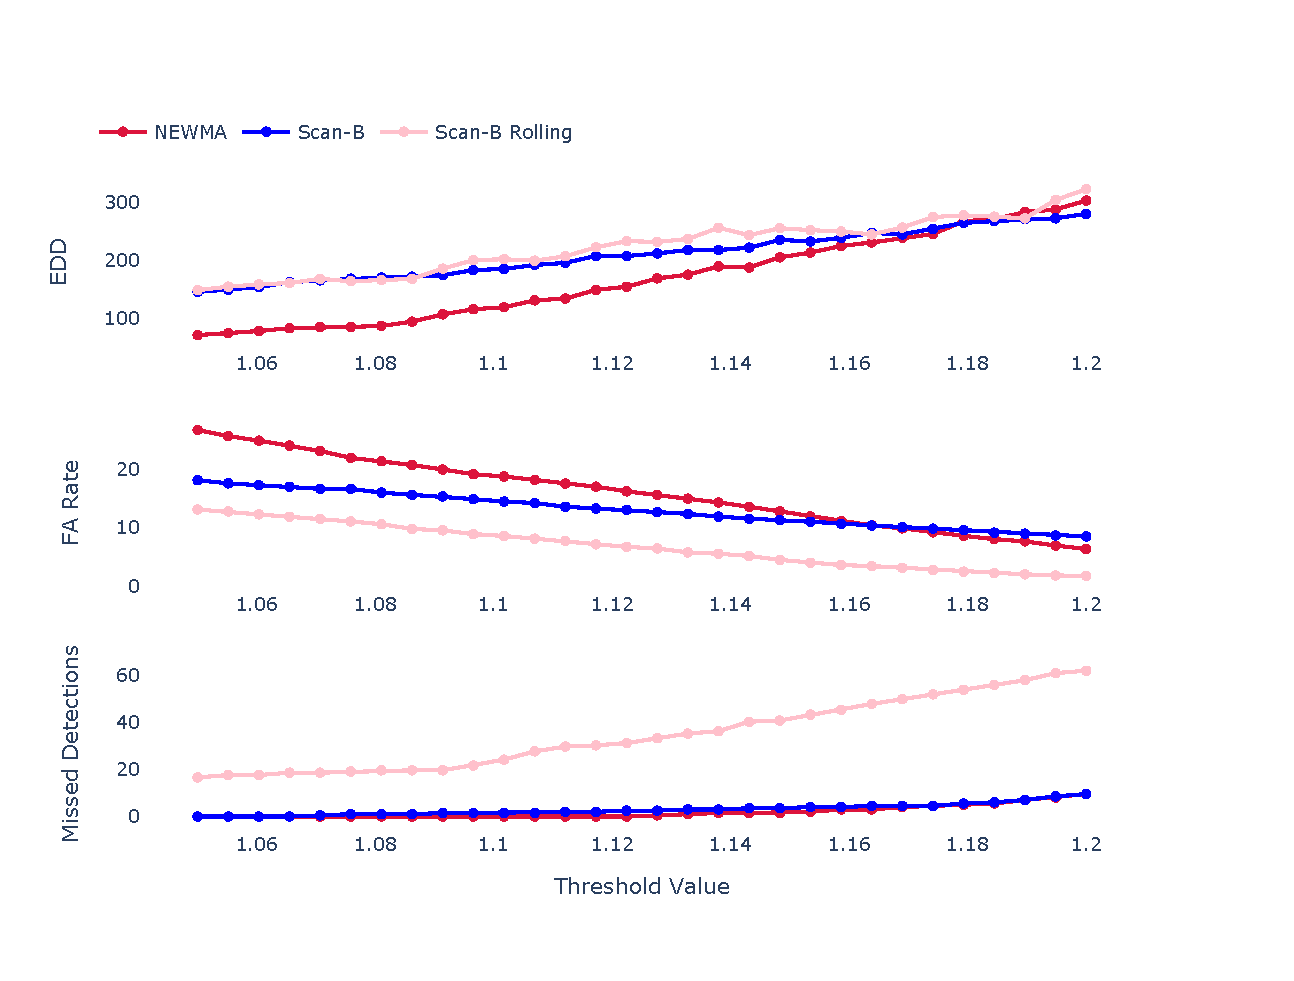
\includegraphics[trim=0cm 1cm 0cm 1cm, clip, width=\textwidth]{gauss_laplace} 
\label{fig:gauss_laplace_results} 
%\medskip
%\tiny
%(top) Daily stock prices (at closing) and (bottom) Daily returns on the stock (evaluated at closing) of Apple Inc. 
\end{center}